\documentclass[a4paper]{report}
\usepackage{hyperref}
\usepackage{lastpage}
\usepackage{fancyhdr}
\usepackage{lineno}
\usepackage{listings}
\usepackage{german}
\usepackage[utf8]{inputenc}
\usepackage{amssymb}
\usepackage{graphicx}
\usepackage{pgf-umlsd-0.7/pgf-umlsd}
\usepackage{tikz}
\usetikzlibrary{shapes,arrows}
\usepackage[final]{pdfpages}
%\newcommand{\genasso}[2]{\begin{minipage}{0.7\textwidth}\begin{normalsize}\begin{flushleft}\textbf{{#1}}\end{flushleft}\end{normalsize}\vspace{-1cm}\begin{flushleft}\begin{small}{#2}\end{small}\end{flushleft}\end{minipage}\\\vspace{0.2cm}}
\pagenumbering{arabic}

\pagestyle{fancy} 
\newcommand{\frontmatter}{\clearpage \cfoot{\thepage\ }
\setcounter{page}{1}
\pagenumbering{Roman}}
\newcommand{\mainmatter}{\clearpage \lhead{\myAuth} \rhead{\myDate} \cfoot{} \rfoot{\thepage\ of \pageref{LastPage}}
\setcounter{page}{1}
\pagenumbering{arabic}}
\newcommand{\backmatter}{\clearpage \rfoot{\thepage\ }
\setcounter{page}{1}
\pagenumbering{alph}}


\newcommand{\makemytitlepage}{\begin{titlepage}
    \begin{center}
        \vspace*{0.8cm}
        
        \Huge
        \textbf{\myTitle}
        
        \vspace{1.5cm}
        
        \Large
        \myAuthor

        \vspace{1.8cm}

        %\begin{large}\textbf{Abstract:} \myAbstract \end{large}
        
\includegraphics[width=6cm]{./IM.jpg}  
        
        \vfill
        
        \huge
        \myAsso
        
        \vspace{1.3cm}
        
        \Large

        %\myDate
        \today
        
    \end{center}
\end{titlepage}}
\newcommand{\myAuth}{Team: *Iron Man*\\B. Pohl, K. Trogant, R. Enseleit, D. Hebecker}
\newcommand{\myAuthor}{Birgit Pohl 574353 (MO. 9-11)\\Kevin Trogant 572451 (Mo. 15-17)\\Ronja Enseleit 572404 (Mo. 15-17)\\Dustin Hebecker 571271 (MO. 9-11)}
\newcommand{\myAsso}{Group: *Iron Man*}
\newcommand{\myDate}{\today}

%%%%%%%%%%%%%%%%%%%%%%%%%%%%%%%%
%%Change Title !!!!!!!!!!!!!!!!!
%%%%%%%%%%%%%%%%%%%%%%%%%%%%%%%%
\newcommand{\myTitle}{Exercise Sheet B}

\begin{document}
\frontmatter
\makemytitlepage
\mainmatter

%%%%%%%%%%%%%%%%%%%%%%%%%%%%%%%%%%%%%%%%%%%%%%%%%%%%%%%%%%
%% Only modify below here  and change myTitle!!!!!!!!!!!!!
%%%%%%%%%%%%%%%%%%%%%%%%%%%%%%%%%%%%%%%%%%%%%%%%%%%%%%%%%%
\section*{Aufgabe 1}
\begin{center}
    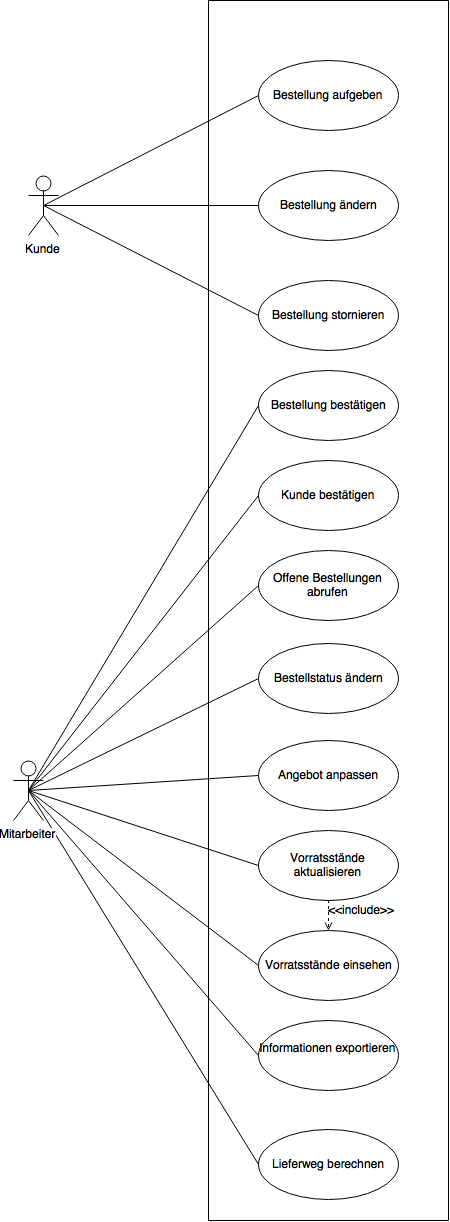
\includegraphics[width=7cm]{use_cases.png}
\end{center}

\newpage
\section*{Aufgabe 2}

%Sample (more here: http://tex.stackexchange.com/questions/207240/drawing-simple-sequence-diagram ) 
\begin{figure}
  \centering
  \begin{sequencediagram}
    \newthread[green!60]{A}{Kunde}
    %\newthread[red!60]{B}{Mitarbeiter}
    \newinst[2]{C}{Web-Server}
    \newinst[2]{D}{DB-Server}
    \newinst[2]{E}{Mail-Server}

    
    \begin{call}{A}{Bestellung Abschicken}{C}{Antwort}
      \begin{call}{C}{Frage Datenbank nach Kunden}{D}{Kunde/Gesperrt/NeuKunde}
      \end{call}
      \begin{sdblock}[black!20!white]{If Kunde}{}
	\begin{call}{C}{Generiere Antwort}{C}{\glqq Bestellung erfolgt \grqq}
	\end{call}
	\begin{call}{C}{Speicher Bestellung}{D}{}
	\end{call}
	\begin{call}{C}{Neue Bestellung}{E}{}
	\end{call}	
      \end{sdblock}
      \begin{sdblock}[black!20!white]{If Gesperrt}{}
	\begin{call}{C}{Generiere Antwort}{C}{\glqq Sie sind gesperrt. Keine Bestellung möglich.\grqq}
	\end{call}
      \end{sdblock}    
      \begin{sdblock}[black!20!white]{If NeuKunde}{}
	\begin{call}{C}{Generiere Antwort}{C}{\glqq Bestellung erfolgt. Ein Bestätigungsanruf folgt.\grqq}
	\end{call}
	\begin{call}{C}{Speicher Bestellung $+$ call flag}{D}{}
	\end{call}
	\begin{call}{C}{Neue Bestellung}{E}{}
	\end{call}
      \end{sdblock}    
    \end{call}
  \end{sequencediagram}
  \caption{Sequenzdiagramm der Bestellungsaufnahme}
\end{figure}


\begin{figure}
  \centering
  \begin{sequencediagram}
    \newthread[red!60]{B}{Mitarbeiter}
    \newinst{C}{Web-Server}
    \newinst{D}{DB-Server}
    \newinst{E}{Mail-Server}
    \newthread[green!60]{A}{Kunde}

   \mess{E}{Neue Bestellung}{B}
   \begin{call}{B}{Zeige Bestellungen}{C}{}
   \end{call}
   \begin{sdblock}[black!20!white]{If call flag}{}
	\begin{call}{B}{Rufe Kunden an}{A}{Bestätigung}
	\end{call}
	\begin{sdblock}[black!20!white]{If not Bestätigung}{}
	  \begin{call}{B}{Entferne Bestellung}{C}{}
	  \end{call}
	\end{sdblock}  
   \end{sdblock}
   \begin{call}{B}{Bearbeite vorherige Bestellungen}{B}{Fertig}
    \begin{call}{A}{Bestellungs Änderung/Löschung}{C}{}
      \begin{call}{C}{Bestellungs Änderung/Löschung}{D}{}
      \end{call}      
    \end{call}
   \end{call}
    \begin{call}{B}{Bearbeite Bestellung}{B}{Fertig}
      \begin{call}{B}{Makiere Bestelleung als in Bearbeitung}{C}{Bestätigung}
	\begin{call}{C}{Makiere Bestelleung als in Bearbeitung}{D}{Bestätigung}
	\end{call}      
      \end{call}
     \begin{sdblock}[black!20!white]{If Bestätigung}{}
      \begin{call}{B}{Mache Pizza(s)}{B}{}
      \end{call}
     \end{sdblock}
    \end{call}
    \mess{B}{Lieferung/Abholung}{A}  
  \end{sequencediagram}
  \caption{Sequenzdiagramm der Bestellungsbearbeitung}
\end{figure}

% submit order
% compare with database
% if new
% store user and set call flag
% if blocked
% reject
% store order in DB send mail to pizza bäcker
% if abort cancel
% if mark in production
% store in db


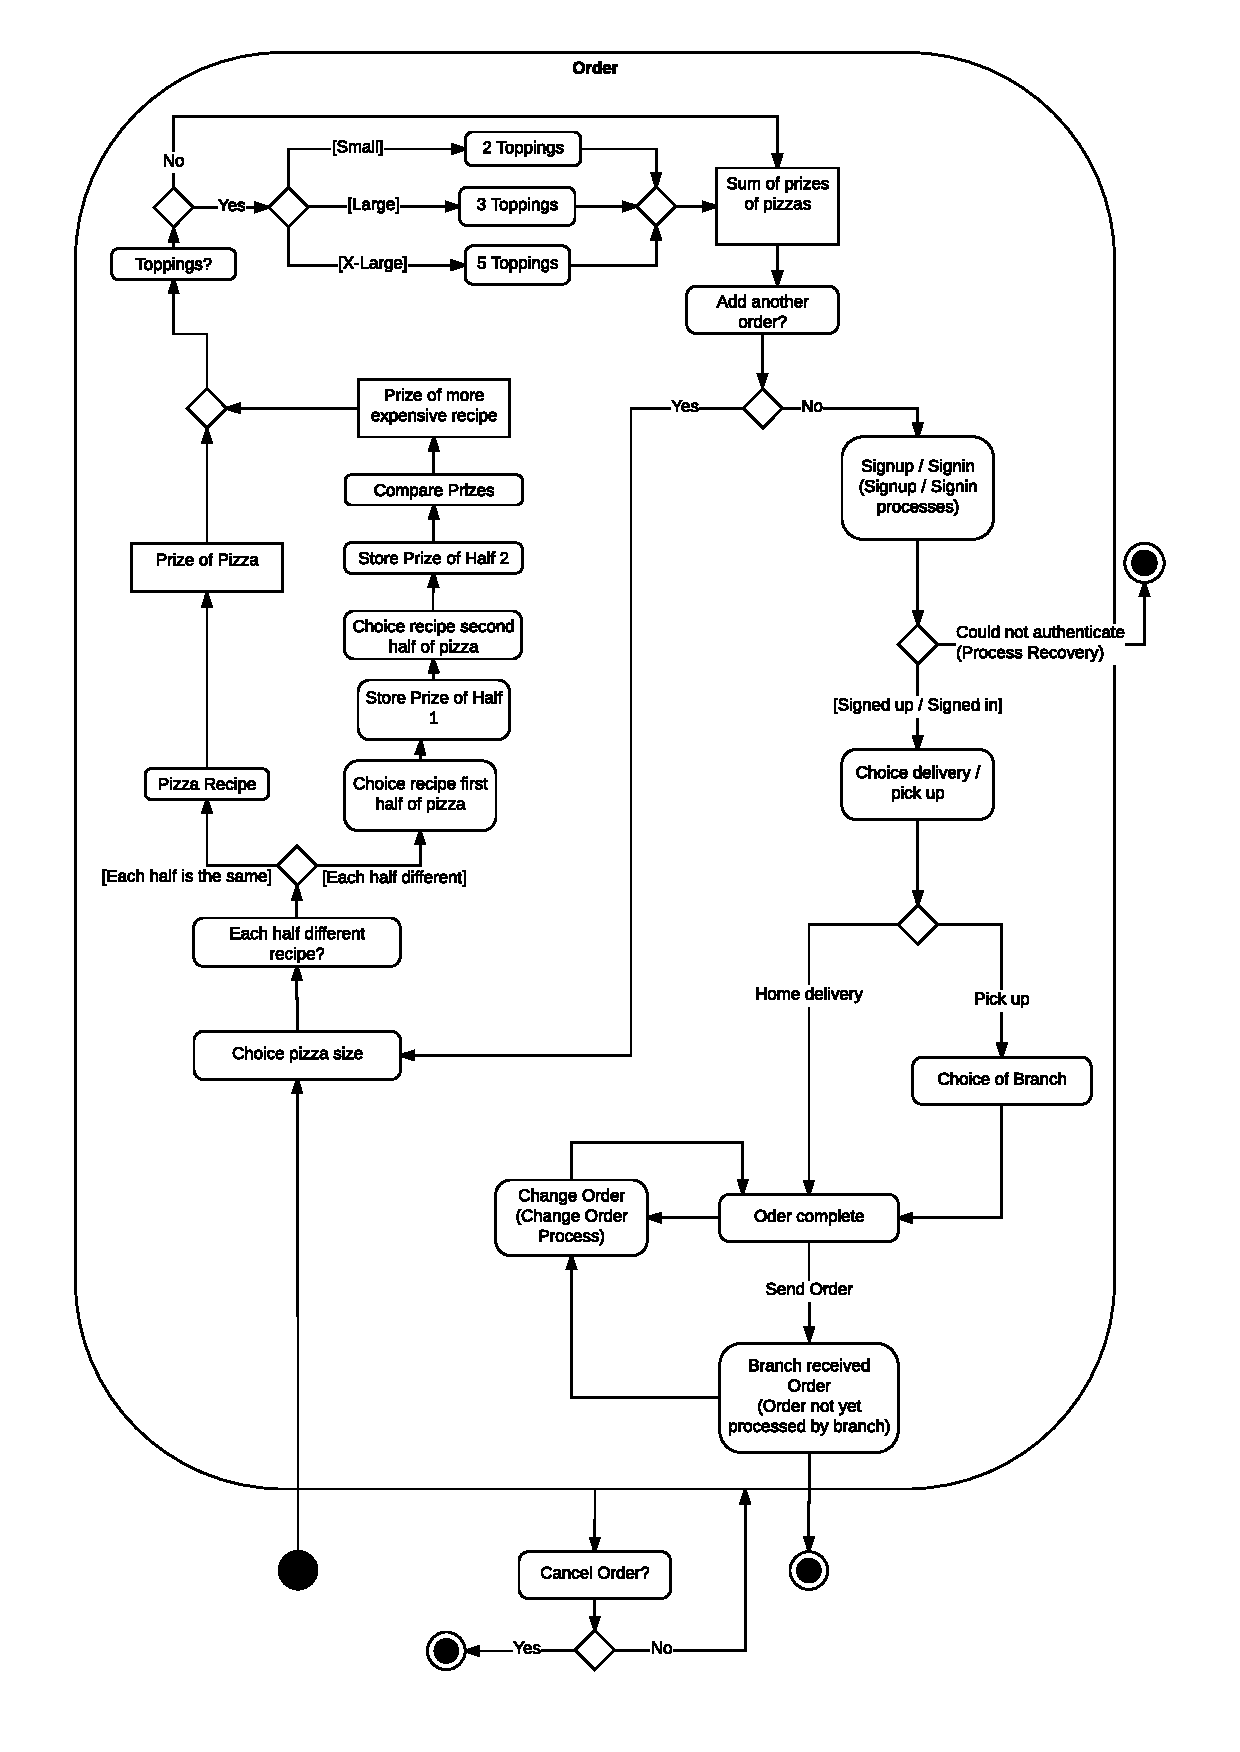
\includepdf[pages=-]{Activitydiagram.pdf}


%\begin{lstlisting}
%Put your code here.
%\end{lstlisting}



\end{document}
